\section{Solution approach}
\begin{flushleft}
The solution to CHEERS is built using RDD principles. Hence the whole solution is divided into multiple classes. Each of this classes have only one specific task to do. The list of the classes are as follows.
\begin{itemize}
  \item Controller class: It calculates angle at vertex and length of overlapping segment.
  \item Root approximation: It calculates the roots of given equation using secant method.
  \item Math Library: It mathematical functions such as power, factorial
  \item Trigonometry: It contains trigonometric function such as Sine and Cos
  \item Output Generator: It generates output in XML format and flat file format
\end{itemize}

When ever the user runs the  program to calculate the overlapping length L, The controller class fetches the radius of circle from the user. Next, it initializes the remaining classes using a wrapper class. wrapper class provide a way to modify or extend the behavior of an existing class without having to modify the class itself. 
\end{flushleft}
\begin{flushleft}
In order to calculate the overlapping length l, we need to first calculate the angle alpha which is angle created with the vertex at the centre point of the left coaster. To do that, we need to find roots of the equation $\alpha - \sin(\alpha) = \frac{\pi}{2}$. 
The roots of this equation is calculated by secant approximation function in rootapproximation class. Secant approximation calls custom Sine function, which in turn use custom factorial and exponent function to calculate the sine value of a given number. 
Here, the sine of a given number is calculated using Maclaurin series. The calculated sin value is then returned secant approximation function. 
The calculated value alpha is returned to Controller class.
\end{flushleft}
\begin{flushleft}
  Next the distance is calculated using the equation $l = 2R\left(1 - \cos\frac{\alpha}{2}\right)$. Similar to sine the cos is calculated using Maclaurin series. Finally, the output is stored as a xml file and the overlapping  length is displayed to the user.
\end{flushleft}
    \pagebreak

  \section{Object Oriented Design}
    \subsection{Sequence Diagram}
      \vspace{1cm}
      \begin{figure}[h!]
        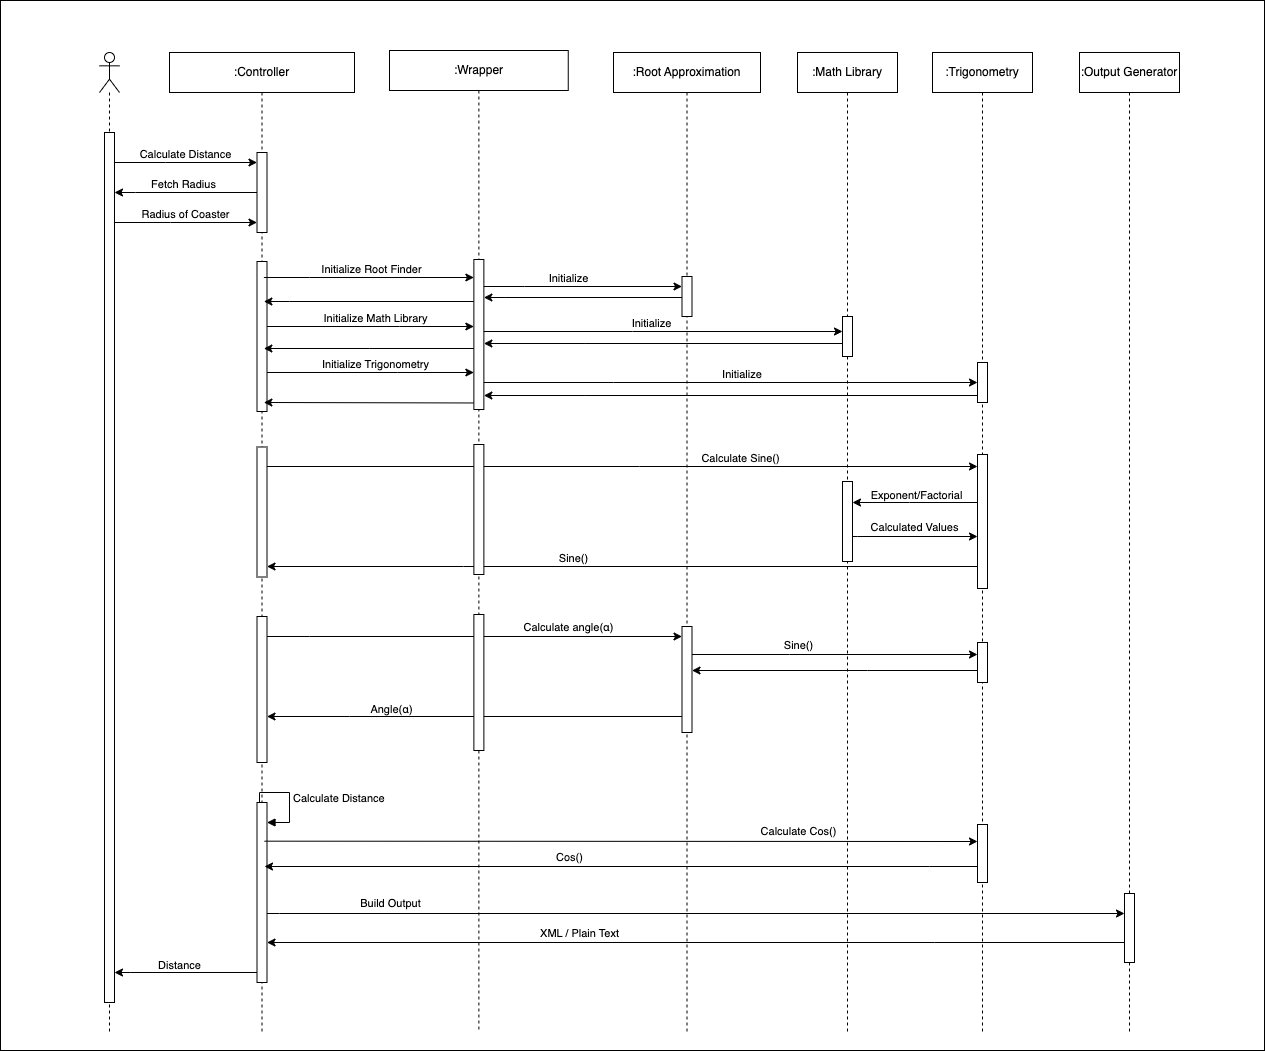
\includegraphics[width=1\linewidth]{resources/cheers-sequence.png}
        \vspace{.5cm}
        \caption{Flow of events for calculating distance}
        \label{fig:Sequence Diagram}
      \end{figure}
      \pagebreak

  \subsection{CRC Cards}
  \begin{figure}[h!]
      \centering
      \begin{tabular}{@{}c@{}}
        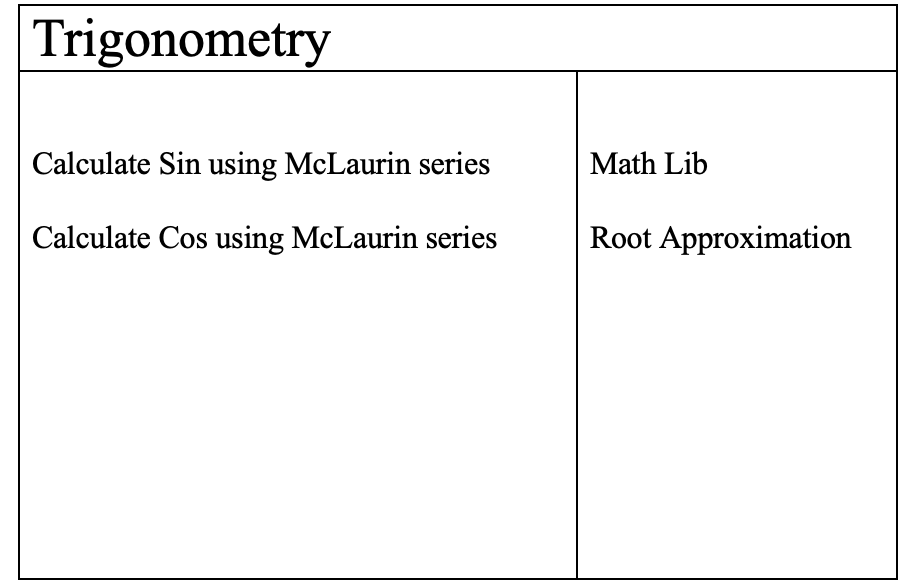
\includegraphics[width=.3\linewidth]{resources/Trigonometry.png} 
          \hspace*{30pt}
        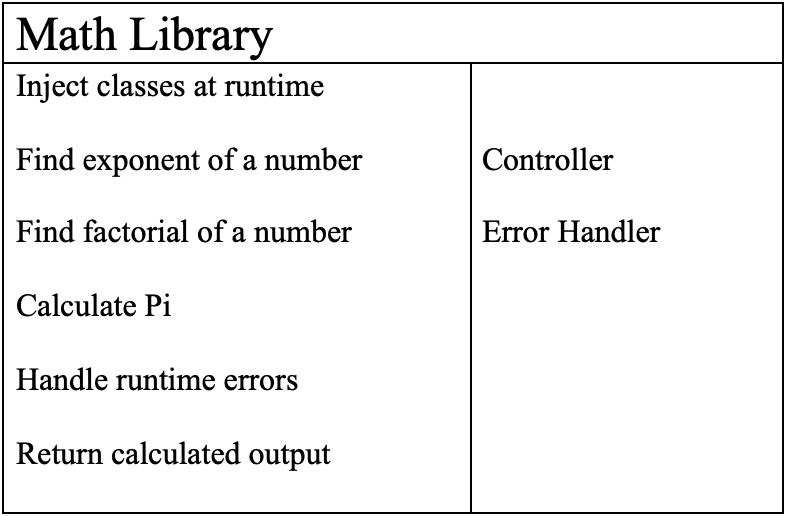
\includegraphics[width=.3\linewidth]{resources/MathLib.png}
      \end{tabular}
    
      \begin{tabular}{@{}c@{}}
          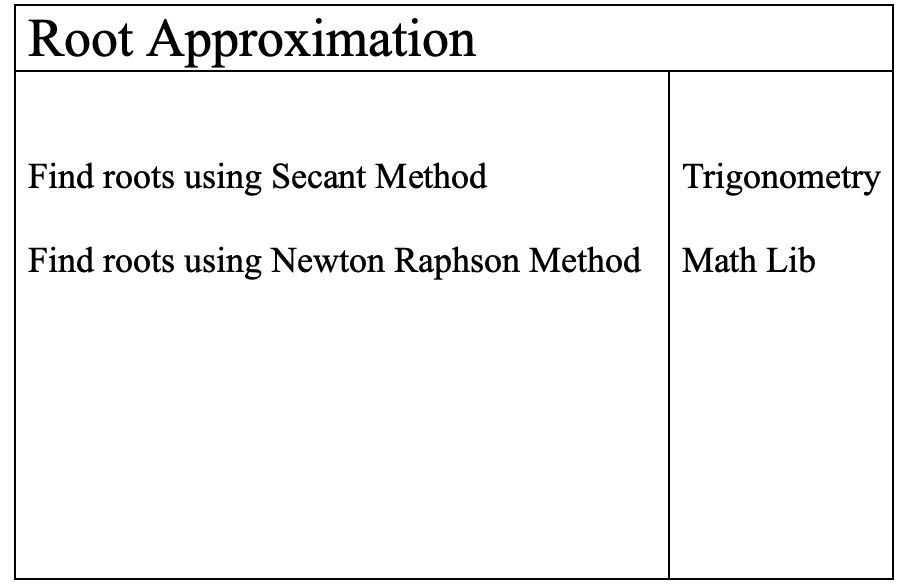
\includegraphics[width=.3\linewidth]{resources/RootApproximation.png} 
            \hspace*{30pt}
          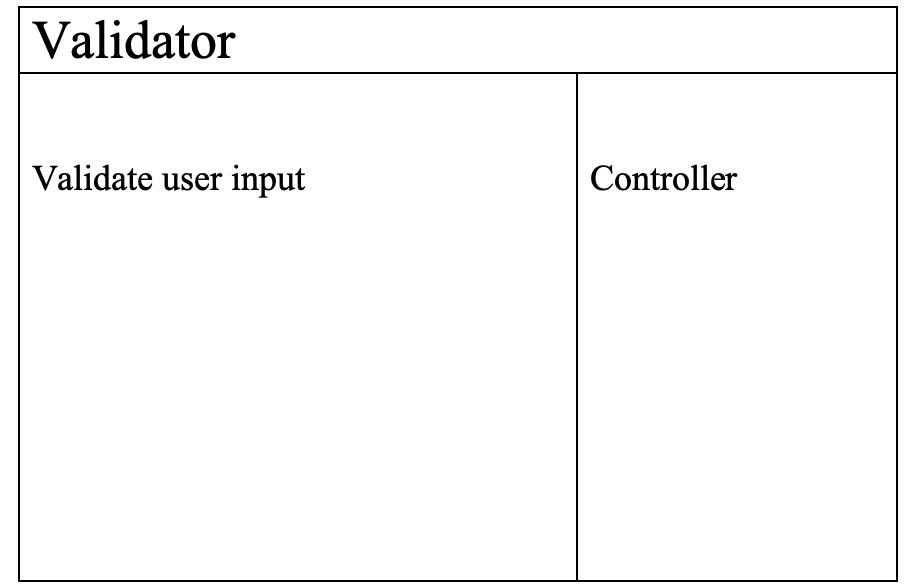
\includegraphics[width=.3\linewidth]{resources/Validator.png}
        \end{tabular}

        \begin{tabular}{@{}c@{}}
          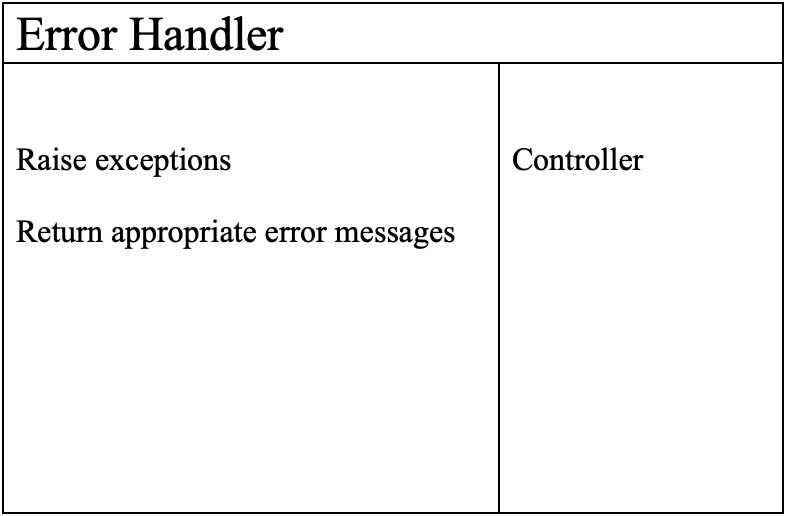
\includegraphics[width=.3\linewidth]{resources/ErrorHandler.png} 
            \hspace*{30pt}
          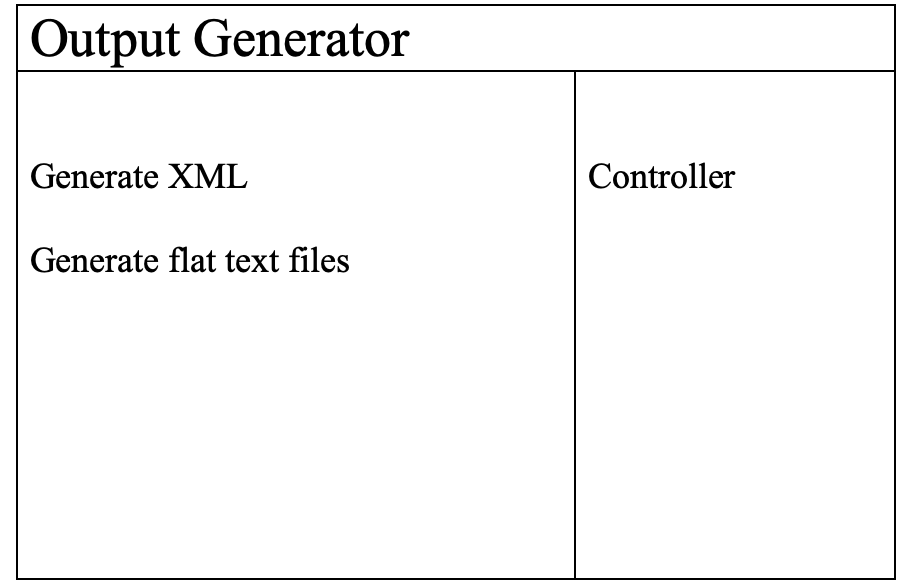
\includegraphics[width=.3\linewidth]{resources/OutputGenerator.png}
        \end{tabular}
        
        \begin{tabular}{@{}c@{}}
          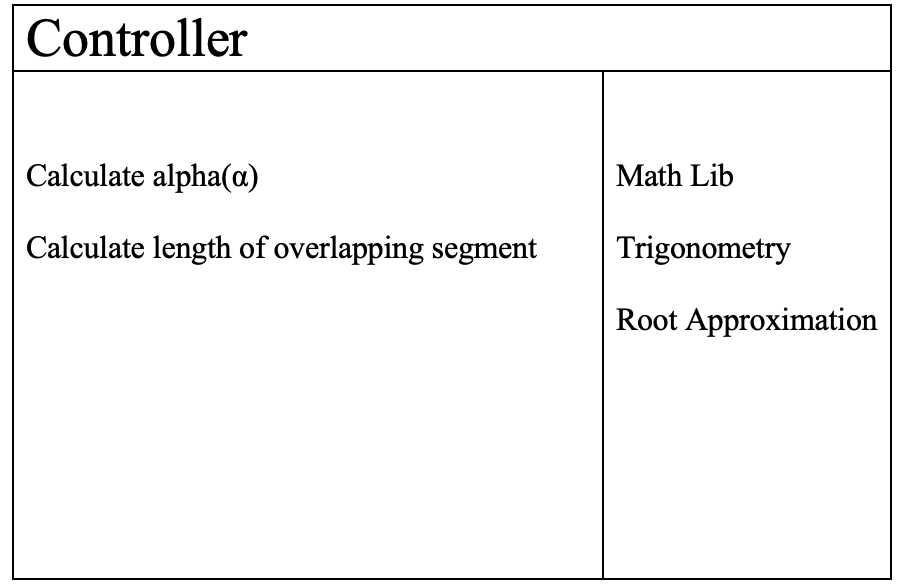
\includegraphics[width=.4\linewidth,height=90pt]{resources/Controller.png}
        \end{tabular}

        \vspace{\floatsep}
      \caption{Overview of CRC Cards for CHEERS}\label{fig:myfig}
  \end{figure}
  \newpage
  \begin{figure}
    \centering
    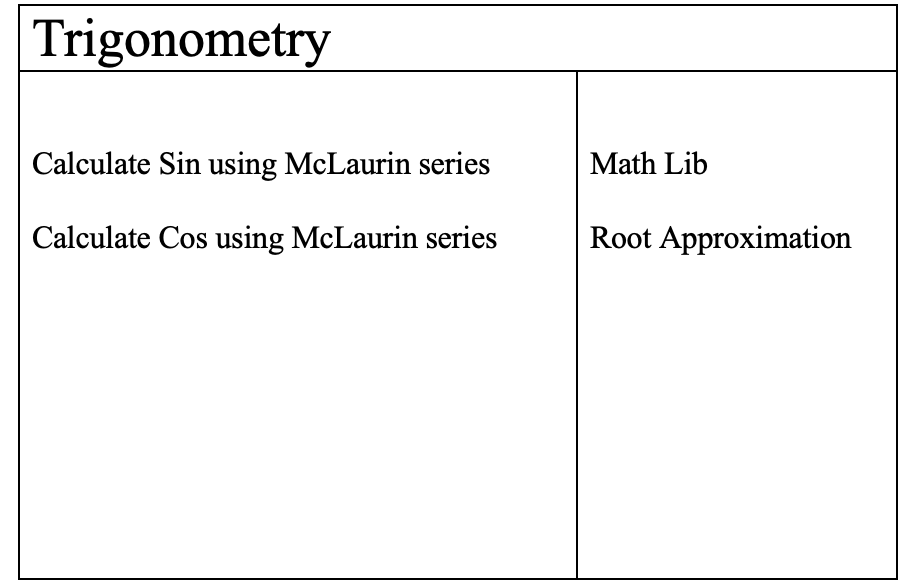
\includegraphics[width=.5\linewidth]{resources/Trigonometry.png}
    \caption{CRC Card of Trignometry Class}\label{fig:trignometry}
    \parbox{1.0\linewidth}{
      Trigonometry class is responsible for calculating Sin and Cos of a given number. Its role is to calculate the sin and cos of a number using McLaurin series to a user defined precision level. It collaborates with MathLib class for accessing the exponential and factorial functions and with Root Approximation class that needs Sin and cos for calculating the roots of the function.
    }
  \end{figure} 
  \begin{figure}
    \centering
    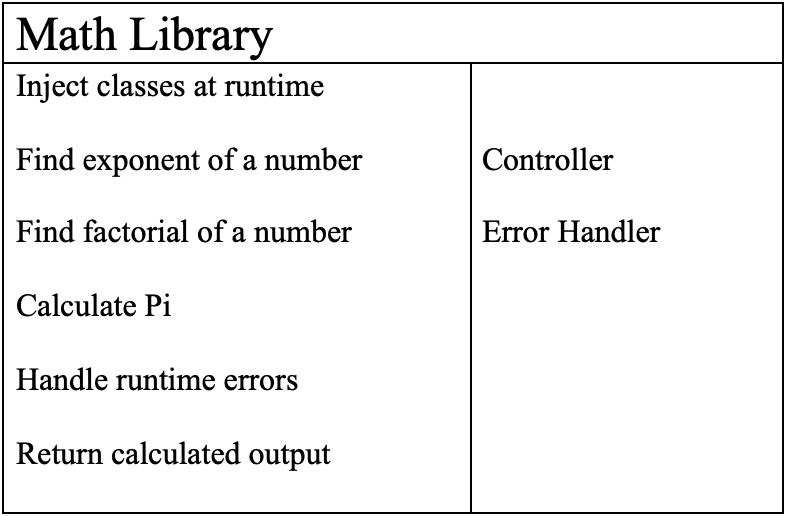
\includegraphics[width=.5\linewidth]{resources/MathLib.png}
    \caption{CRC Card of MathLib Class}\label{fig:mathlib}

    \parbox{1.0\linewidth}{
      The responsibility of Math Lib class is to provide the function definition of Mathematical functions such as factorial, power of a given number. Its role is to calculate the value of PI using Leibniz formula, factorial and power of a given number using recursion. It collaborates with trigonometry, Root approximation and error handling class. This class is chosen because each of the function in the class is reused multiple times throughout the project. So instead of rewriting the code we reuse it.

    }
  \end{figure}
  \begin{figure}
    \centering
    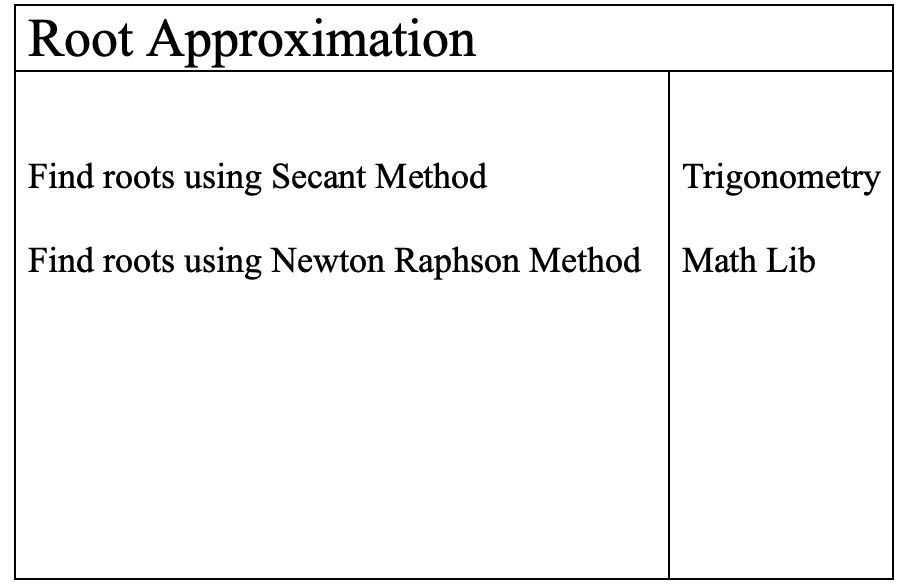
\includegraphics[width=.5\linewidth]{resources/RootApproximation.png}
    \caption{CRC Card of Root Approximation Class}\label{fig:rootapprox}

    \parbox{1.0\linewidth}{
      The root approximation class it the core of the entire project. It contains two functions that calculate the roots of the given equation. It collaborates with Trigonometry and Math Lib classes as the contain necessary functions used for root approximation. As we always try to reduce the coupling with multiple classes and increase the cohesion within the class, we chose this class as to perform only one task of calculating the roots of equation.
      }
  \end{figure} 
  \begin{figure}
    \centering
    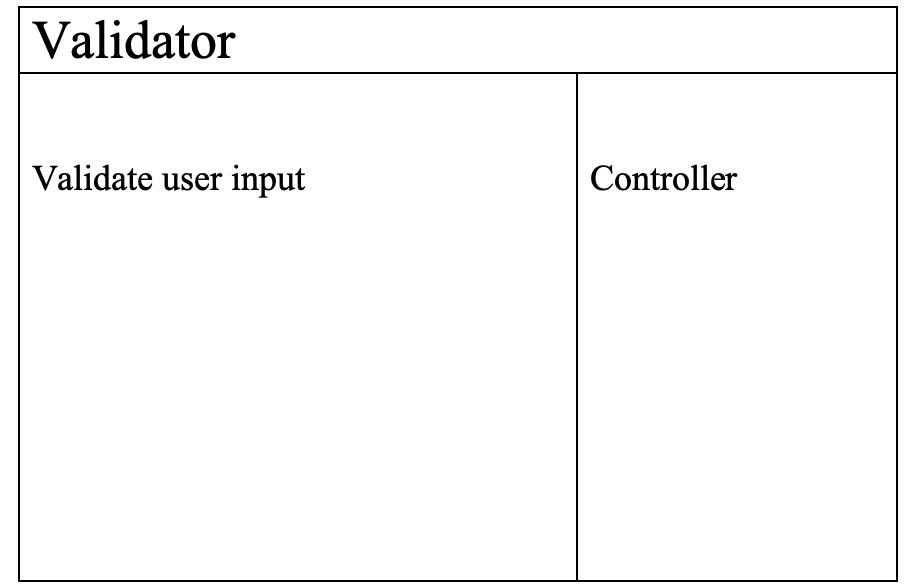
\includegraphics[width=.5\linewidth]{resources/Validator.png}
    \caption{CRC Card of Validator Class}\label{fig:validator}
    \parbox{1.0\linewidth}{
      The role of input validator class is to make sure that the data received from the user is appropriate format. It makes sure that the data given by the user is a positive integer. If the user enters invalid data, it prompts the user to provide valid data.
      }
  \end{figure}  
  \begin{figure}
    \centering
    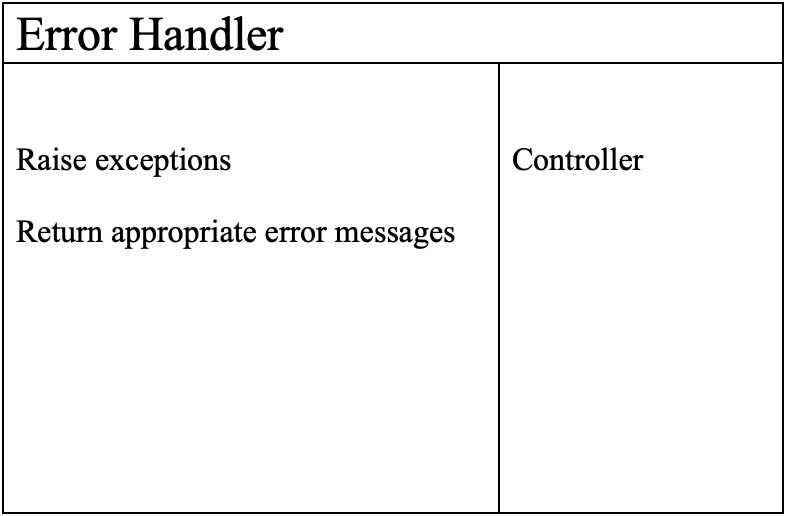
\includegraphics[width=.5\linewidth]{resources/ErrorHandler.png}
    \caption{CRC Card of ErrorHandler Class}\label{fig:error}

    \parbox{1.0\linewidth}{
      The role of error handler class is to handle errors that are generated. It collaborates with controller class. The main responsibility this class is to handle the errors generated and return a appropriate error message that is human understandable. The rationale for choosing this class is to define and handle all possible errors that are generated in the process of calculating angle alpha and length l.
      }

  \end{figure}
  \begin{figure}[h]
    \centering
    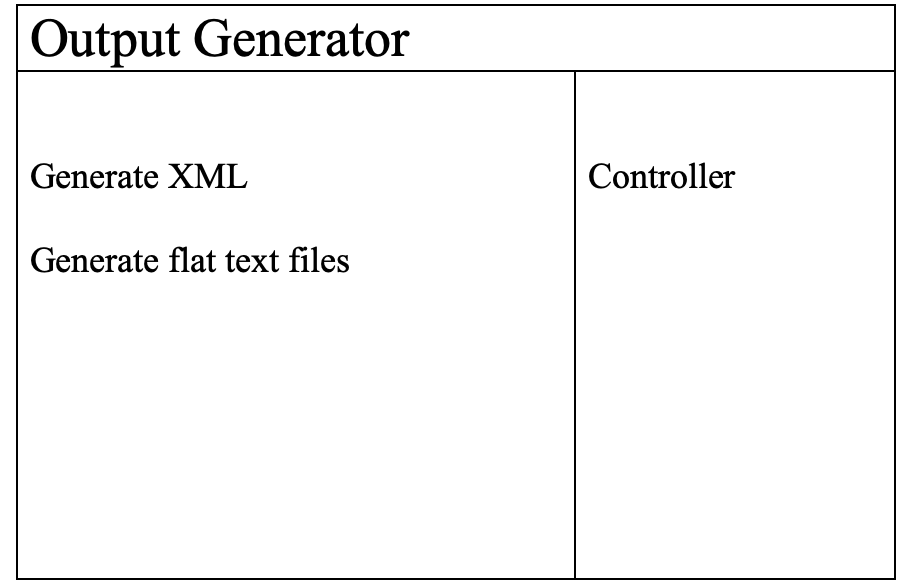
\includegraphics[width=.5\linewidth]{resources/OutputGenerator.png}
    \caption{CRC Card of OutputGenerator Class}\label{fig:output}
    \parbox{1.0\linewidth}{
      The main role Output Generator class is to generate XML files. It stores the radius of the circle and the overlapping length l in form of a xml object. The rational behind choosing this class is to make sure that the processing and output are separated so that any changes to the output format doesnot affect the processing capabilities. This reduces the coupling between the classes.
      }

  \end{figure}
 
  \begin{figure}[h]
    \centering
    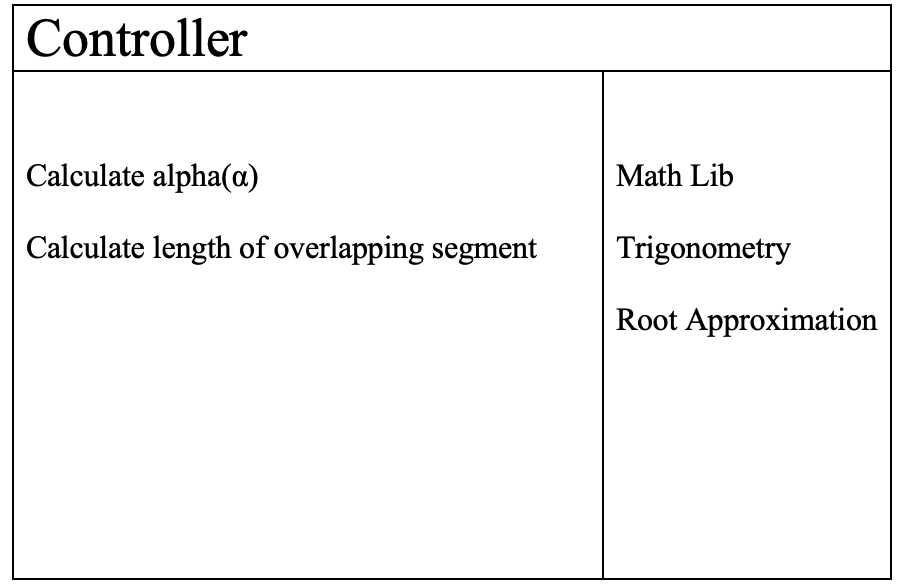
\includegraphics[width=.5\linewidth]{resources/Controller.png}
    \caption{CRC Card of Controller Class}\label{fig:control}
    \parbox{1.0\linewidth}{
      The main role of this class is to calculate $\alpha$,the angle with vertex at the center of the left circle. It also calculates the length of overlapping segment. To do this, it collaborates with other classes which includes MathLib, Trigonometry and root approximation. Each of these classes are contains various mathematical functions such as Sin, Cos and secant approximation that are required for calculating the angle $\alpha$ and length l.
      }
  \end{figure}
